\chapter{Simulations}
	\section{principe des simulations}

		\subsection{analytiques}

Les simulateurs Analytiques ne simulent pas de manière réaliste le déplacement des particules mais  utilisent des approximation fortes pour résoudre les problèmes de manière analytiques..

Dans le cas de l'imagerie TEP, la simulation analytique revient à réaliser des projections du volume TEP dans l'espace du sinogramme en utilisant les pour simuler les désintégrations 

		\subsection{monte carlo}

Les simulations Monte-Carlo vont avoir une approche probabiliste en modélisant la trajectoire de chaque photon indépendamment. Le nom de Monte-Carlo fait allusion aux jeux de hasards pratiqués dans la ville du même nom.

Dans le cadre de l'imagerie TEP, le modèle probabiliste est appliqué depuis l'émission puis le parcours du positon, l'annihilation, ainsi que les interactions et la probabilité de détection des photons dans les détecteurs. 

Le simulateur le plus connu actuellement est GATE~\cite{jan2004gate}, qui se base sur le jeu d'outils de simulation d'interactions particule/matière geant4~\cite{allison2006geant4}. L'utilisation de cette librairie très pointue permet à GATE de prendre en compte avec une grande précision l'ensemble des phénomènes physiques. Cependant, cela se fait au détriment des temps de calculs. Une nouvelle version de GATE est en cours de développement pour accélérer les temps de simulation.<Voir>




		\subsection{MC accélérés}

	\section{simulateurs disponibles}

	\section{processus de simulation avec SORTEO}

Pour reproduire les données fournies par les systèmes cliniques TEP, les simulateurs Monte-Carlo simulent les désintégrations une par une et suivent les sous-produits dans les tissus jusqu'aux détecteurs. Étant donné qu'un examen TEP génère plusieurs millions de désintégrations, les temps de simulations deviennent très rapidement insurmontables. PET-SORTEO dispose de plusieurs heuristiques qui permettent d'accélérer les simulations. Cependant il faut tout de même plusieurs dizaines d'heures pour simuler une image.

Le logiciel PET-SORTEO réalise une simulation TEP accélérée afin de conserver des temps de calculs raisonnables. Il réalise tout d'abord une simulation Monte-Carlo réaliste à faible statistique, dont il se se sert pour estimer le taux de photons émis par une région et arrivant sur un détecteur. Cela permet de prendre en compte les effets du temps mort dans les simulations (photons non pris en compte par les détecteurs à cause d'une saturation du capteur) sans réaliser une simulation complète. Cette information permet par la suite de ne plus simuler de manière exacte les chemins des photons. Les photons diffusés et directs seront par exemple simulés séparément. De cette manière, pendant la simulation des directs, si un des photons est atténué, l'autre peut être détruit directement.

Puis il réalise les simulations proprement dites en simplifiant les interactions : par exemple, si un des deux photons est absorbé, l'autre est détruit et une nouvelle désintégration est générée.

	\section{Contribution à SORTEO}

\begin{itemize}
    \item Le code original du simulateur SORTEO n'étais pas adapté aux architectures réseau du centre de calcul de l'in2p3 : Le système de communication entre les processus consommait trop de ressources réseau. J'ai donc réalisé des modifications en profondeur du code pour séparer le simulateur en plusieurs entités, chacune réalisant une seule partie du travail :

    \begin{enumerate}
        \item Estimation des paramètres nécessaires à la simulation accélérée par simulation Monte-Carlo pur (lancé pour chaque processus)
        \item Combinaison des résultats Monte-Carlo
        \item Simulation simplifiée des désintégrations (lancé pour chaque processus)
        \item Combinaison des désintégrations détectées pour chaque processus dans un seul fichier de données
    \end{enumerate}

    \item Le code original ne permettait pas la sauvegarde de l'information temporelle de chaque évènement détecté. Or cette information est nécessaire aux méthodes de correction du mouvement du mouvement respiratoire telles que celles proposées par F. Lamare. Le format d'enregistrement des simulations par défaut est le sinogramme, qui est une matrice 3D indiquant pour chaque ligne de réponse le nombre de désintégrations détectées. Il a donc fallu reprendre le code source du logiciel PET-SORTEO pour l'adapter à un format de sortie compatible. 
\end{itemize}

\subsection{Gestion des lits}

Le découpage des simulations en lits est nécessaire pour simuler de manière réaliste des acquisitions médicales. Or le logiciel de reconstruction avec correction de mouvement ne prenait pas du tout en compte la possibilité de découper les images en lits. 

J'avais supposé lorsque j'avais commencé à utiliser le logiciel que son créateur avait utilisé cette possibilité, mais il utilisait dans ses simulations une caméra virtuelle qui couvrait tout le patient. Cela a augmenté la complexité du système de reconstruction, car je devais réaliser autant d'estimation de mouvement qu'il y avait de lits.

\todo{gestion des lits .. peut-être plus dans la partie apport perso}

\section{Reconstruction des images}

Nous avons utilisé le logiciel de reconstruction fourni par le LaTIM dans le cadre d'un partenariat, crée et utilisé par Frédéric Lamare pour ses travaux sur la correction du mouvement respiratoire~\cite{lamare2007list}.

Il est capable de reconstruire les images acquises en données séquentielles à l'aide de l'algorithme OPL-EM décrit en \ref{lab:OPLEM}. La reconstruction permet de prends en compte la correction de l'atténuation, mais n epermet pas la correction des coïncidences aléatoires ni des diffusés. Nous avons donc choisit de simplifier le problème en considérant que la correction de ces deux effets était parfaite, en n'incluant pas dans les données séquentielles les photons diffusés ou les coïncidences aléatoires.

Nous avons choisit de corriger les images en utilisant la méthode de correction post reconstruction décrite en \ref{lab:corrPostRecon} ainsi que la correction par modification de la matrice système décrite en \ref{lab:corrMatSyst}. La première est déjà implémentée sur les imageur GE (technologie motionFree), tandis que la seconde est activement étudiée en recherche. 

\section{Estimation de mouvement}

L'estimation de mouvement est réalisée uniquement à partir des données TEP et des informations de synchronisation respiratoire. 

\subsection{Principe de l'estimation de mouvement}

L'estimation de mouvement est réalisée selon le principe énoncé en~\ref{lab:estimMvtTEP4D} :
\begin{enumerate}
 \item Les données simulées des 4 cycles sont additionnées pour chaque instant respiratoire.
 \item Les images correspondant à chaque instant du cycle respiratoire sont reconstruites à partir de ces données en utilisant l'algorithme OPL-EM.
 \item Les 8 images générées sont utilisées pour calculer le mouvement respiratoire : Les images des temps 2 à 8 sont recalées sur l'image de référence (numéro 1), ce qui associe à chaque instant respiratoire un champ de déformation.
\end{enumerate}

\subsection{Estimation des performances}

Les images correspondant à chaque instant respiratoire sont reconstruites séparément, avec des paramètres différents de ceux utilisés pour reconstruire les images complètes. En effet, la quantité de données disponible pour la reconstruction est 8 fois plus faible que celle utilisée pour réaliser les reconstructions d'images complètes. De plus, nous cherchons à optimiser la qualité de l'estimation de mouvement. C'est pour ces raisons que nous avons réalisé une autre étude pour estimer les paramètres de reconstruction optimaux. 

Pour évaluer la performance de chaque jeu de paramètre, nous avons utilisé la vérité terrain pour créer une image d'évaluation pour l'image de référence, ainsi qu'une autre pour l'image ``respirante``. Les images d'évaluations sont crées à partir des fantômes de référence en assignant aux organes étudiés (foie et poumon) une valeur de 1, et une valeur plus importante pour les lésions, comme indiqué dans la figure~\ref{lab:perfsFctIterReg}.a). 

\begin{figure}
\centering
\begin{tabular}{c c}
	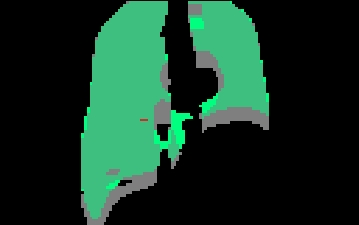
\includegraphics[width=5cm]{images/sansCorrection} & 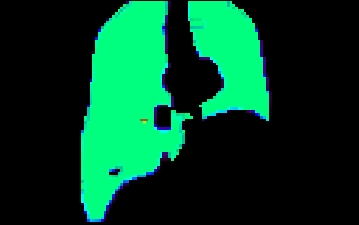
\includegraphics[width=5cm]{images/avecCorrection} \\
	a) Cartes non recalées				& b) Cartes recalées
\end{tabular}
\caption[Illustration du recalage obtenu]{Illustration de la pertinence du recalage obtenu à partir de l'estimation de mouvement réalisée sur les images. En vert l'image de référence et en gris l'image correspondant au temps correspondant à la différence la plus importante. }
\label{lab:perfsFctIterReg}
\end{figure}

L'image d'évaluation correspondant à l'image ''respirante`` est alors recalées sur l'image de référence à l'aide du champ de mouvement élastique calculé précédemment. J'évalue ensuite la qualité du recalage en réalisant une somme des différences au carré entre les deux images d'évaluation~\ref{lab:perfsFctIterReg}.b).


\subsection{Optimisation des paramètres de reconstruction}


Nous avons évalué la performance des reconstructions pour les paramètres suivants :
\begin{description}
 \item[Nombre d'itérations complètes :] Le nombre de sous-ensembles est toujours de 5, mais nous faisons varier le nombre d'itérations commplètes de 1 à 7, ce qui représente un nombre d'itérations totales de 5 à 40.
 \item[Présence ou absence de régularisation pendant la reconstruction :] Une régularisationde \todo{verif}5mm  est appliquée ou non à chaque itération complète.
\end{description}

Les résultats sont présentés dans la figure~\ref{lab:perfsFctIterReg}. Ils montrent clairement que la régularisation entraîne une baisse de performance, et que la meilleure estimation de mouvement est réalisée pour une reconstruction de 3 itérations complètes avec 5 subsets.

\begin{figure}
\centering
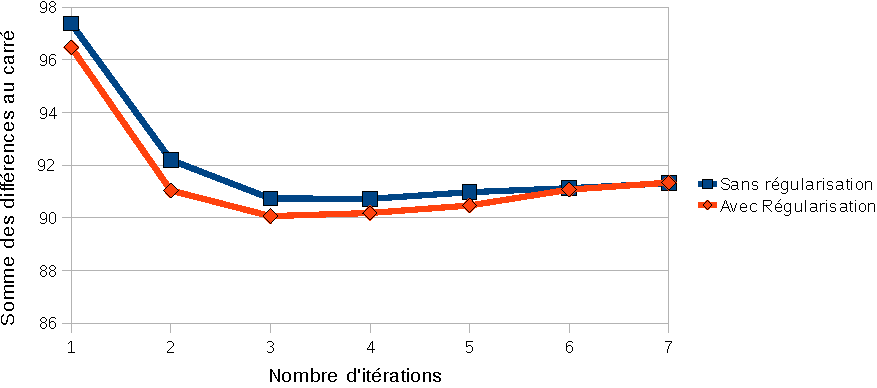
\includegraphics[width=10cm]{images/perfsRecalageFctIter_crop}
\caption[Performances de l'estimation de mouvement en fonction de la réguilarisation]{Performances de l'estimation de mouvement en fonction du nombre d'itérations complètes de la reconstruction selon la présence ou l'absence de régularisation pendant la reconstruction. Plus la valeur en ordonnées (mesure de différence) est faible, meilleure et la performance}
\label{lab:perfsFctIterReg}
\end{figure}



\begin{figure}
\centering
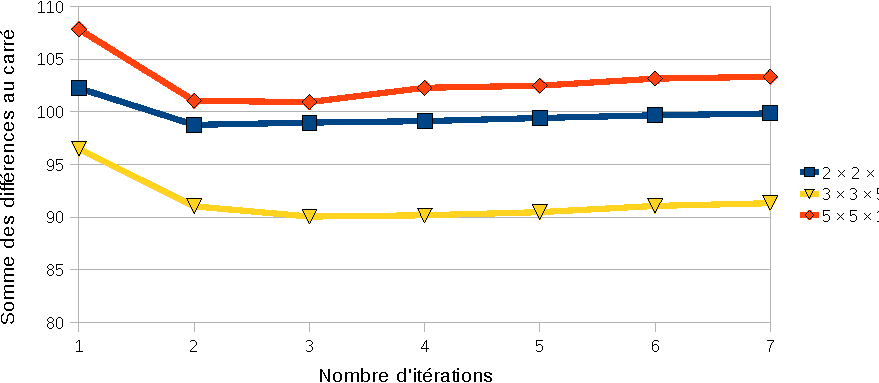
\includegraphics[width=10cm]{images/perfsRecalageFctIter-grid_crop}
\caption[Performances de l'estimation de mouvement en fonction de la taille de la grille de recherche]{Performances de l'estimation de mouvement en fonction du nombre d'itérations complètes de la reconstruction selon la taille de la grille utilisée pour l'estimation de mouvement}
\label{lab:perfsFctIterTaille}
\end{figure}


\subsection{paramètres de reconstruction}

